% ============================================================
%  Chapter 5 — Solving Problems That Have Multiple Solution
%              Characteristics (Multi-Objective Optimisation)
%  Nature-Inspired Optimisation for Delivery Problems (2022)
%  Self-contained Beamer lecture slides
% ============================================================
\documentclass[aspectratio=169,10pt]{beamer}

\usetheme{Madrid}
\usecolortheme{seahorse}

\usepackage{amsmath,amssymb}
\usepackage{booktabs}
\usepackage{tabularx}
\usepackage{array}
\usepackage{graphicx}
\usepackage{xcolor}
\usepackage{listings}
\usepackage{multicol}
\usepackage{tikz}
\usetikzlibrary{arrows.meta,shapes,positioning}
\usepackage{hyperref}
\usepackage{microtype}

\graphicspath{{figures/}}

% ─── listings style ────────────────────────────────────────────────────────
\lstset{
  language=Python,
  basicstyle=\ttfamily\scriptsize,
  numbers=left,
  numberstyle=\tiny\color{gray},
  frame=single,
  backgroundcolor=\color{gray!7},
  keywordstyle=\color{blue!80!black}\bfseries,
  commentstyle=\color{green!50!black}\itshape,
  stringstyle=\color{orange!80!black},
  breaklines=true,
  showstringspaces=false,
  xleftmargin=1.5em,
  framexleftmargin=1.5em,
  tabsize=4,
}

% ─── footline ──────────────────────────────────────────────────────────────
\setbeamertemplate{footline}[frame number]
\setbeamertemplate{navigation symbols}{}

% ─── title info ────────────────────────────────────────────────────────────
\title[Chapter 5 — Multi-Objective Delivery]{%
  Chapter 5: Solving Problems That Have\\
  Multiple Solution Characteristics}
\subtitle{Nature-Inspired Optimisation for Delivery Problems (2022)}
\author{N.~Urquhart}
\institute{Natural Computing Series, Springer}
\date{2022}

% ============================================================
\begin{document}
% ============================================================

\begin{frame}
  \titlepage
\end{frame}

% ────────────────────────────────────────────────────────────
\begin{frame}{Chapter Overview}
% ────────────────────────────────────────────────────────────
  This chapter extends our optimisation toolkit from single-objective to
  \textbf{multi-objective problems}.  In practice, a delivery planner rarely
  cares about just one thing: cost, time, emissions, and number of vehicles all
  matter simultaneously, and improving one often worsens another.  The chapter
  introduces the concepts and algorithms needed to navigate these trade-offs.

  \begin{block}{Sections at a Glance}
    \begin{enumerate}
      \item \textbf{5.1} Last Mile Deliveries — the business context and
            why multiple objectives arise naturally.
      \item \textbf{5.2} Vehicle Routing with Time Windows (VRPTW) —
            adding time constraints to the VRP.
      \item \textbf{5.3} A Case Study: FabFoods Home Delivery — cost model,
            representation, decoding, and implementation.
      \item \textbf{5.4} Finding Trade-Offs Using Pareto Dominance —
            multi-objective evolutionary algorithm and results.
      \item \textbf{5.5} Exploring Many-Dimensional Fronts — parallel
            coordinates for visualising and filtering high-D Pareto fronts.
      \item \textbf{5.6} Conclusions.
    \end{enumerate}
  \end{block}

  \begin{alertblock}{Key Insight}
    Evolutionary algorithms are \emph{naturally suited} to multi-objective
    optimisation because they maintain a \emph{population} of solutions — many
    trade-off points can be discovered in a single run.
  \end{alertblock}
\end{frame}

% ============================================================
\section{5.1 Last Mile Deliveries}
% ============================================================

\begin{frame}[allowframebreaks]{5.1 Last Mile Deliveries — Context}

  The \textbf{last mile} is the final step in the supply chain: the movement
  of a parcel or grocery order from a local depot or fulfilment centre directly
  to the consumer's home.  The term ``last mile'' is used even though the
  actual distance may be many kilometres.

  The on-demand economy has caused an explosive growth in business-to-consumer
  (B2C) deliveries.  Data from the UK Office of National Statistics (ONS)
  shows that online purchases rose from \textbf{7.7\%} of UK retail sales in
  July 2011 to \textbf{26\%} in July 2021, reaching \textbf{36\%} in
  December 2020.  The vast majority of those purchases require a home
  delivery.

  \begin{figure}
    \centering
    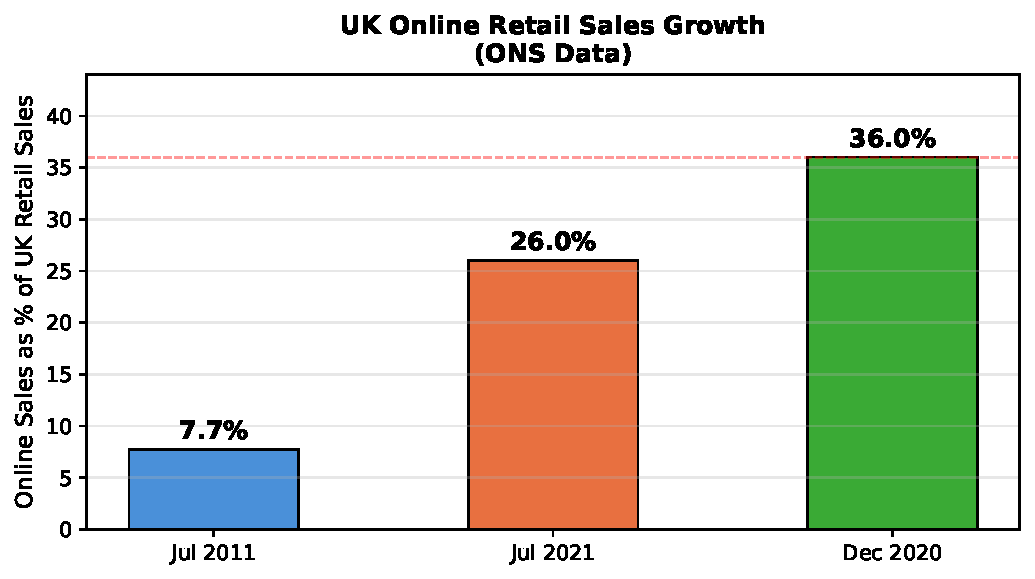
\includegraphics[width=0.55\textwidth]{fig_last_mile_growth.pdf}
    \caption{UK online retail sales as a percentage of total retail sales.
             Data from ONS (2021).}
  \end{figure}

\framebreak

  \begin{block}{Why Is This Hard? — The Four Objective Dimensions}
    When planning a typical last-mile delivery operation, the planner must
    balance at least four competing dimensions:
    \begin{itemize}
      \item \textbf{Financial} — capital costs (purchasing vehicles), running
            costs (fuel, maintenance), energy costs, and staff wages.  These
            pull in opposite directions: fewer, longer routes cut vehicle
            overhead but increase driver wages.
      \item \textbf{Environmental} — CO$_2$ emissions and road congestion.
            Emissions depend on distance driven, load weight, and vehicle
            type (van vs cargo bike vs walking courier).
      \item \textbf{Customer Service} — customers specify \emph{delivery time
            windows}; missing a window generates complaints or failed
            deliveries.
      \item \textbf{Delivery Technology} — the choice of vehicle type (vans,
            cargo bikes, walking couriers) affects cost, range, and capacity
            simultaneously.
    \end{itemize}
  \end{block}

  These four dimensions interact in complex ways.  For example, using more
  vehicles reduces individual route duration (good for time-window
  compliance) but raises the number of routes (bad for financial cost).
  There is no single solution that is simultaneously best in every dimension
  --- instead, there exist \textbf{trade-off solutions} that are
  \emph{Pareto optimal}: you cannot improve one objective without worsening
  at least one other.

  \begin{alertblock}{Key Insight}
    Because many real-world objectives conflict with each other, the correct
    output of a multi-objective solver is \emph{not} a single answer but
    rather a \textbf{set of Pareto-optimal solutions} from which a human
    decision-maker can choose.
  \end{alertblock}

\end{frame}

% ============================================================
\section{5.2 Vehicle Routing with Time Windows}
% ============================================================

\begin{frame}[allowframebreaks]{5.2 Vehicle Routing with Time Windows (VRPTW)}

  The \textbf{Vehicle Routing Problem with Time Windows (VRPTW)} adds time
  constraints to the classic VRP: every customer $i$ has a time window
  $[e_i, l_i]$ (where $e_i$ is the \emph{earliest} acceptable arrival time
  and $l_i$ is the \emph{latest}).  Deliveries must be made within those
  windows, and each customer also requires a \emph{service time} $s$ — the
  time spent at the customer's door unloading goods.

  \begin{figure}
    \centering
    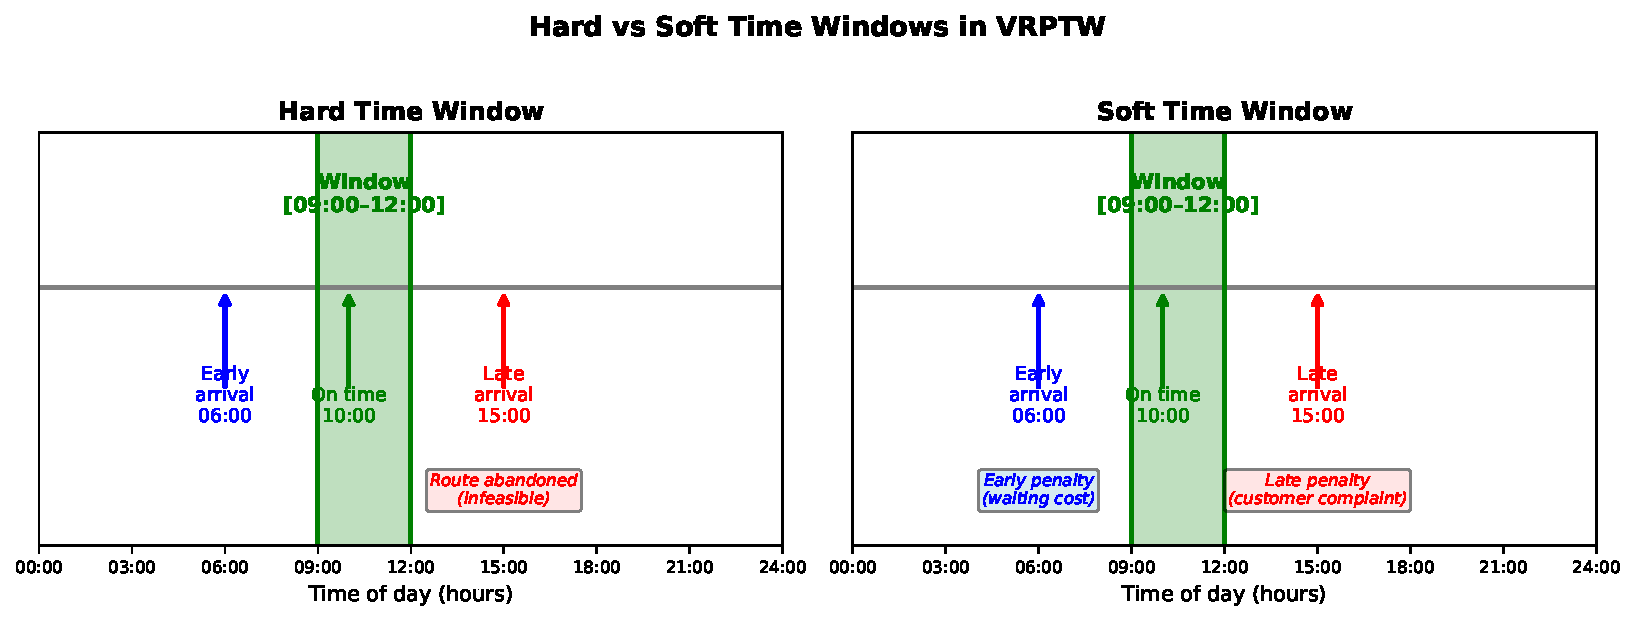
\includegraphics[width=0.85\textwidth]{fig_time_windows.pdf}
    \caption{Hard time window (left) vs soft time window (right).
             In a hard window, a late arrival makes the route infeasible.
             In a soft window, a late arrival incurs a penalty but is still
             accepted.}
  \end{figure}

\framebreak

  \begin{block}{The VRP Family Tree}
    VRPTW is one member of a large family of vehicle routing variants:
    \begin{itemize}
      \item \textbf{CVRP} (Capacitated VRP) — each vehicle has a load
            capacity $Q$ (Q).
      \item \textbf{VRPTW} (VRP with Time Windows) — hard or soft
            time-window constraints.
      \item \textbf{CVRPTW} (Capacitated + Time Windows) — the most
            commonly studied variant.
      \item \textbf{DVRP} (Dynamic VRP) — new orders arrive during the
            working day.
      \item \textbf{VRPPDTW} (VRP with Pickup and Delivery + Time Windows) —
            vehicles both collect and deliver.
      \item \textbf{VRPB} (VRP with Backhauls) — a subset of customers are
            collection points.
    \end{itemize}
  \end{block}

  \begin{figure}
    \centering
    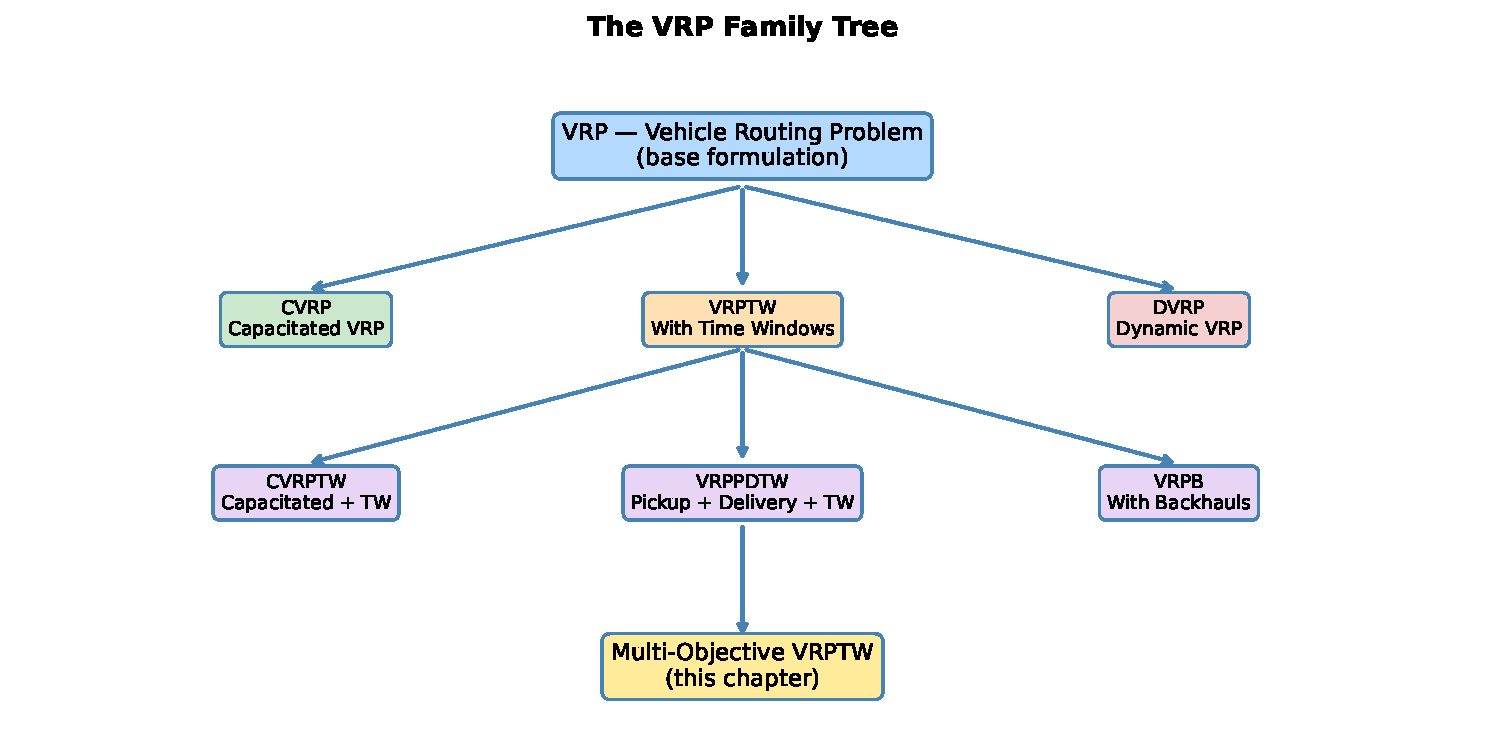
\includegraphics[width=0.65\textwidth]{fig_vrp_family.pdf}
    \caption{Hierarchy of VRP variants.  The focus of this chapter is
             the multi-objective VRPTW at the bottom.}
  \end{figure}

\framebreak

  \begin{block}{Formal Definition of Hard and Soft Time Windows}
    Let vehicle $v$ arrive at customer $i$ at time $a_i$ (a, for arrival).
    \begin{itemize}
      \item \textbf{Hard time window}: if $a_i < e_i$ (e, early bound),
            the vehicle \emph{waits} at the customer's door until $e_i$ —
            this is called \emph{waiting time}.  If $a_i > l_i$ (l, late
            bound), the route is declared \textbf{infeasible} and the
            decoder must start a fresh route for this customer.
      \item \textbf{Soft time window}: early or late arrivals are allowed
            but incur a \textbf{penalty cost} that is added to the
            objective function.  The route remains feasible.
    \end{itemize}
  \end{block}

  \begin{exampleblock}{Worked Example: Waiting Time}
    Suppose a vehicle leaves the depot at 08:30 and the travel time to
    customer 5 is 8 minutes.  The vehicle arrives at 08:38.  However,
    customer 5's window is $[12\!:\!00,\ 13\!:\!00]$.  The vehicle must
    \textbf{wait} at customer 5's door from 08:38 until 12:00 (a wait of
    3 hours and 22 minutes).  Service takes 5 minutes, so the vehicle
    \textbf{departs} customer 5 at 12:05.  This waiting time counts toward
    the total route duration (and thus staff cost).
  \end{exampleblock}

  The service time $s$ is typically a constant for all customers.  In the
  FabFoods case study below, $s = 5$ minutes per customer.

  \begin{alertblock}{Key Insight}
    Tighter time windows force more routes: if a customer's window closes
    before the vehicle can reach them from the previous stop, a new route
    must be started.  This is why a 1-hour time window can roughly
    \textbf{double} the number of routes (and hence the cost) compared to a
    14-hour window.
  \end{alertblock}

\end{frame}

% ============================================================
\section{5.3 A Case Study: FabFoods Home Delivery}
% ============================================================

\begin{frame}[allowframebreaks]{5.3 Case Study — FabFoods Home Delivery}

  \textbf{FabFoods} is a fictional (but realistic) online grocer based on the
  \textbf{Augerat benchmark set}, a standard academic test suite for VRPTW
  problems.  The problem uses \emph{crates} as the unit of demand: each
  customer orders a certain number of crates of grocery items, and each
  vehicle holds a fixed number of crates.

  FabFoods wants to minimise \textbf{four objectives simultaneously}:

  \begin{columns}[t]
    \column{0.48\textwidth}
    \begin{block}{Four Objectives}
      \begin{enumerate}
        \item \textbf{Distance} — total distance of all routes combined
              (in kilometres or route-distance units).
        \item \textbf{Time} — total duration of all routes combined
              (in minutes), including travel, waiting, and service.
        \item \textbf{Routes} — total number of routes, which determines
              how many vehicles are in use.
        \item \textbf{Cost/Crate} — the financial cost per crate delivered
              (see the cost model below).
      \end{enumerate}
    \end{block}

    \column{0.48\textwidth}
    \begin{alertblock}{Why Four Objectives?}
      Distance minimisation saves fuel but may use many routes.  Time
      minimisation reduces wage bills but may increase distance.  Minimising
      routes reduces vehicle overhead but forces longer individual routes.
      Cost/Crate ties everything together into a single financial metric —
      but optimising it alone ignores environmental or customer-service
      impacts.  Only a Pareto approach can show all the trade-offs.
    \end{alertblock}
  \end{columns}

\framebreak

  \begin{block}{The FabFoods Cost Model}
    The total cost of a delivery plan is computed in three steps:

    \[
      \textit{vehicleCost} = (\textit{noRoutes} \times \text{VEHFIXED})
        + (\textit{totalDistance} \times \text{VEHRUNNING})
    \]

    Here, \textit{noRoutes} is the number of routes (one vehicle per route);
    VEHFIXED $= 164$ (pounds, the fixed cost of putting one vehicle on the
    road for the day); \textit{totalDistance} is the total kilometres driven;
    VEHRUNNING $= 0.117$ (pounds per kilometre, the per-km running cost).

    \[
      \textit{staffCost} = \textit{totalTime} \times \text{STAFF\_RATE}
    \]

    Here, \textit{totalTime} is the total route duration in hours;
    STAFF\_RATE $= 12$ (pounds per hour per member of staff).  One driver
    is assumed per vehicle, paid from departure to return.

    \[
      \textit{solutionCost} = \textit{vehicleCost} + \textit{staffCost}
    \]

    \[
      \textit{costPerCrate} = \frac{\textit{solutionCost}}{\textit{totalDemand}}
    \]

    Here, \textit{totalDemand} is the total number of crates to be delivered.
  \end{block}

\framebreak

  \begin{exampleblock}{Worked Example: Cost Calculation}
    Suppose a solution has 3 routes with a total distance of 200 km, a total
    duration of 6 hours, and there are 50 crates to deliver.

    \smallskip
    \textbf{Step 1 — Vehicle cost:}
    \[
      \textit{vehicleCost} = 3 \times 164 + 200 \times 0.117
                           = 492 + 23.40 = \pounds 515.40
    \]

    \textbf{Step 2 — Staff cost:}
    \[
      \textit{staffCost} = 6 \times 12 = \pounds 72.00
    \]

    \textbf{Step 3 — Total and per-crate:}
    \[
      \textit{solutionCost} = 515.40 + 72.00 = \pounds 587.40
    \]
    \[
      \textit{costPerCrate} = \frac{587.40}{50} = \pounds 11.75 \text{ per crate}
    \]

    If a tighter time window forces one additional route (4 routes total),
    the vehicle cost rises to $4 \times 164 + 200 \times 0.117 = \pounds 679.40$,
    and the cost per crate rises to $\frac{679.40 + 72.00}{50} = \pounds 15.03$.
    A single extra route adds roughly \pounds 3.28 per crate.
  \end{exampleblock}

  \begin{figure}
    \centering
    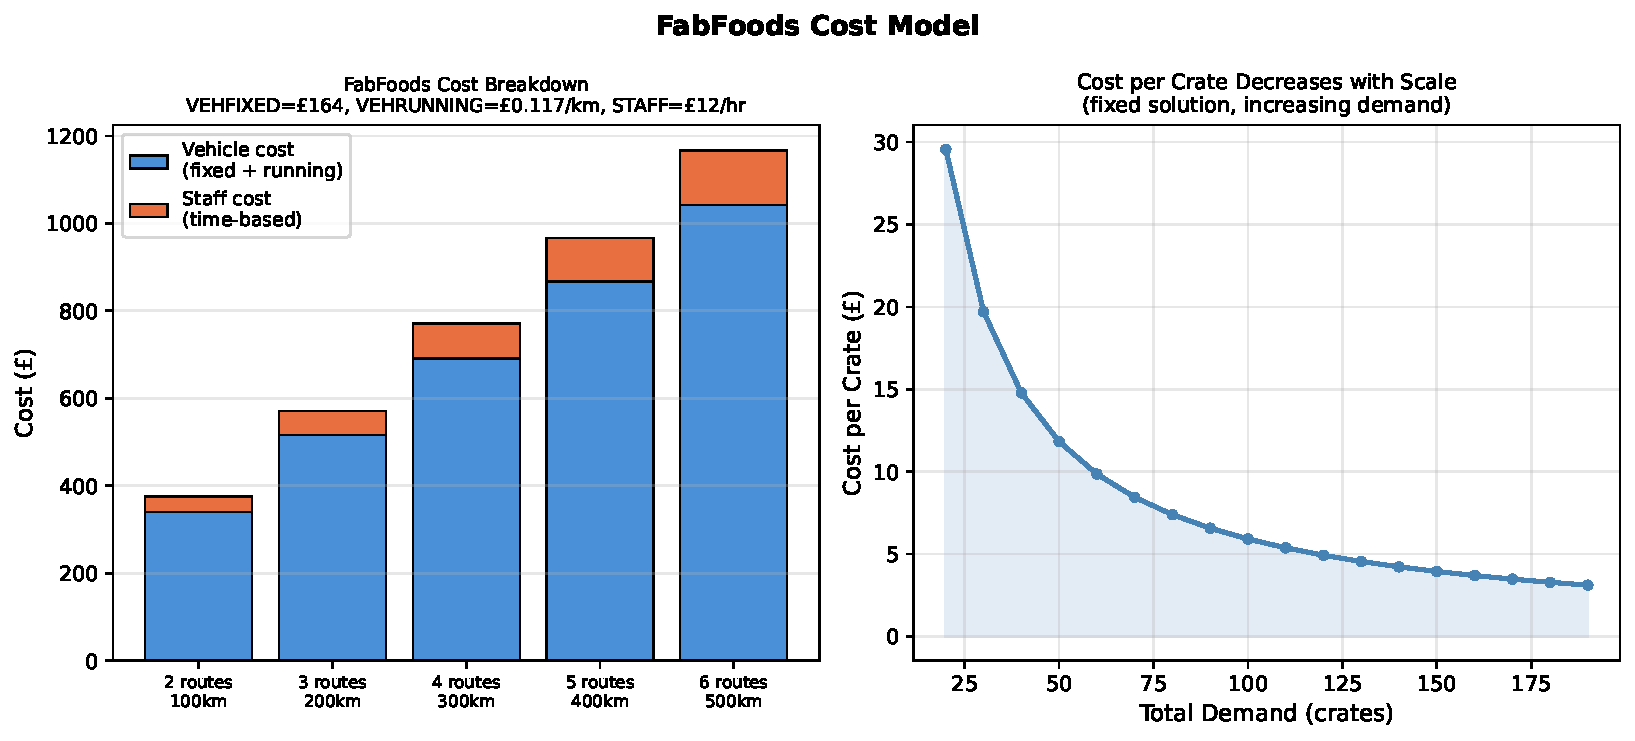
\includegraphics[width=0.88\textwidth]{fig_cost_model.pdf}
    \caption{Left: cost breakdown into vehicle and staff components as the
             number of routes grows.  Right: cost per crate decreases with
             larger total demand — economies of scale.}
  \end{figure}

\framebreak

  \begin{block}{Representation and Decoding}
    The same permutation representation used for the basic CVRP (from
    Chapter 2) is extended here to include time windows.  A solution
    (genotype) is an ordered list of customer identifiers, each paired with
    a Boolean \emph{new-route flag}.  The decoder translates this list into
    a set of routes (phenotype) while respecting both capacity and time
    windows.

    The decoding algorithm works as follows:
    \begin{enumerate}
      \item Start a new route (route 1) and add the first customer in the
            genome.
      \item Calculate the \textbf{arrival time} at that customer.  If arrival
            is before the window opens ($a_i < e_i$), record a wait; the
            vehicle departs at $e_i + s$ (where $s$ is service time).
      \item For each subsequent customer in the genome:
        \begin{itemize}
          \item Compute arrival time from the current position.
          \item If arrival would be after the window closes ($a_i > l_i$),
                \textbf{start a new route} for this customer.
          \item If the new-route flag is \texttt{true}, start a new route
                regardless of feasibility.
          \item If adding the customer would exceed vehicle capacity,
                start a new route.
        \end{itemize}
      \item Repeat until all customers are assigned.
    \end{enumerate}
  \end{block}

\framebreak

  \begin{exampleblock}{Worked Example: Decoding a Genome (from the Book, p.88--89)}
    We have 8 customers with the following time windows and demands:

    \begin{center}
    \small
    \begin{tabular}{crrr}
      \toprule
      Customer & Window Start & Window End & Demand (crates) \\
      \midrule
      1 & 09:00 & 10:00 & 5 \\
      2 & 09:00 & 10:00 & 5 \\
      3 & 11:00 & 12:00 & 10 \\
      4 & 13:00 & 14:00 & 10 \\
      5 & 12:00 & 13:00 & 5 \\
      6 & 10:00 & 11:00 & 5 \\
      7 & 11:00 & 12:00 & 5 \\
      8 & 13:00 & 14:00 & 5 \\
      \bottomrule
    \end{tabular}
    \end{center}

    Vehicle capacity is 20 crates; service time is 5 minutes; depot departs
    at 08:30.

    \medskip
    The genome is:
    \[
      \underbrace{5}_{\text{F}},\;
      \underbrace{2}_{\text{F}},\;
      \underbrace{4}_{\text{F}},\;
      \underbrace{8}_{\text{F}},\;
      \underbrace{1}_{\text{F}},\;
      \underbrace{7}_{\textbf{T}},\;
      \underbrace{3}_{\text{F}},\;
      \underbrace{6}_{\text{F}}
    \]
    (\textbf{T} = start a new route; \textbf{F} = continue current route)
  \end{exampleblock}

\framebreak

  \begin{exampleblock}{Decoding Step-by-Step}
    \textbf{Step 1 — Customer 5, Route 1.}
    Depot departs at 08:30; travel time to customer 5 is 8 min, so the vehicle
    arrives at 08:38.  But customer 5 is not available until 12:00, so the
    vehicle \textbf{waits} until 12:00 and departs at 12:05.
    Route 1: \texttt{5 @ 12:00}

    \medskip
    \textbf{Step 2 — Customer 2.}
    Earliest possible arrival from customer 5 is $12:05 + 15\,\text{min} = 12:20$.
    But customer 2's window \emph{closes} at 10:00.  Arrival is too late
    ($12:20 > 10:00$), so customer 2 must go on a \textbf{new Route 2},
    departing from the depot at 08:50, arriving at 09:00 (within the window).
    Route 2: \texttt{2 @ 09:00}

    \medskip
    \textbf{Steps 3--4 — Customers 4 and 8 added to Route 2.}
    Both fit within Route 2's schedule and within capacity (5+10+5=20).
    Route 2: \texttt{2 @ 09:00, 4 @ 13:00, 8 @ 13:25}

    \medskip
    \textbf{Step 5 — Customer 1.} Route 2 is at capacity; a new Route 3 is started.
    Route 3: \texttt{1 @ 09:00}

    \medskip
    \textbf{Step 6 — Customer 7.} Gene flag is \textbf{T} (true), so a new Route 4
    is \emph{forced} regardless of feasibility.
    Route 4: \texttt{7 @ 11:00, 3 @ 11:17}

    \medskip
    \textbf{Step 7 — Customer 6.} Added to new Route 5 (Route 4 is done).
    Route 5: \texttt{6 @ 10:00}

    \medskip
    \textbf{Final phenotype (5 routes):}
  \end{exampleblock}

\framebreak

  \begin{exampleblock}{Final Decoded Solution}
    \small
    \begin{center}
    \begin{tabular}{lllll}
      \toprule
      Route 1 & Route 2 & Route 3 & Route 4 & Route 5 \\
      \midrule
      D * 12:52 & D * 08:50 & D * 08:48 & D * 10:55 & D * 09:40 \\
      5 @ 13:00 & 2 @ 09:00 & 1 @ 09:00 & 7 @ 11:00 & 6 @ 10:00 \\
      D @ 13:17 & 4 @ 13:00 & D @ 09:17 & 3 @ 11:17 & D @ 10:13 \\
                & 8 @ 13:25 &           & D @ 11:34 &           \\
                & D @ 13:53 &           &           &           \\
      \bottomrule
    \end{tabular}
    \end{center}
    \medskip
    (D = Depot; * = departs at; @ = arrives at)
    \medskip

    An additional optimisation is possible: one vehicle can serve Route 3
    then Route 5 then Route 4, and finally Route 1, provided sufficient
    time exists for re-loading between runs.
  \end{exampleblock}

  \begin{figure}
    \centering
    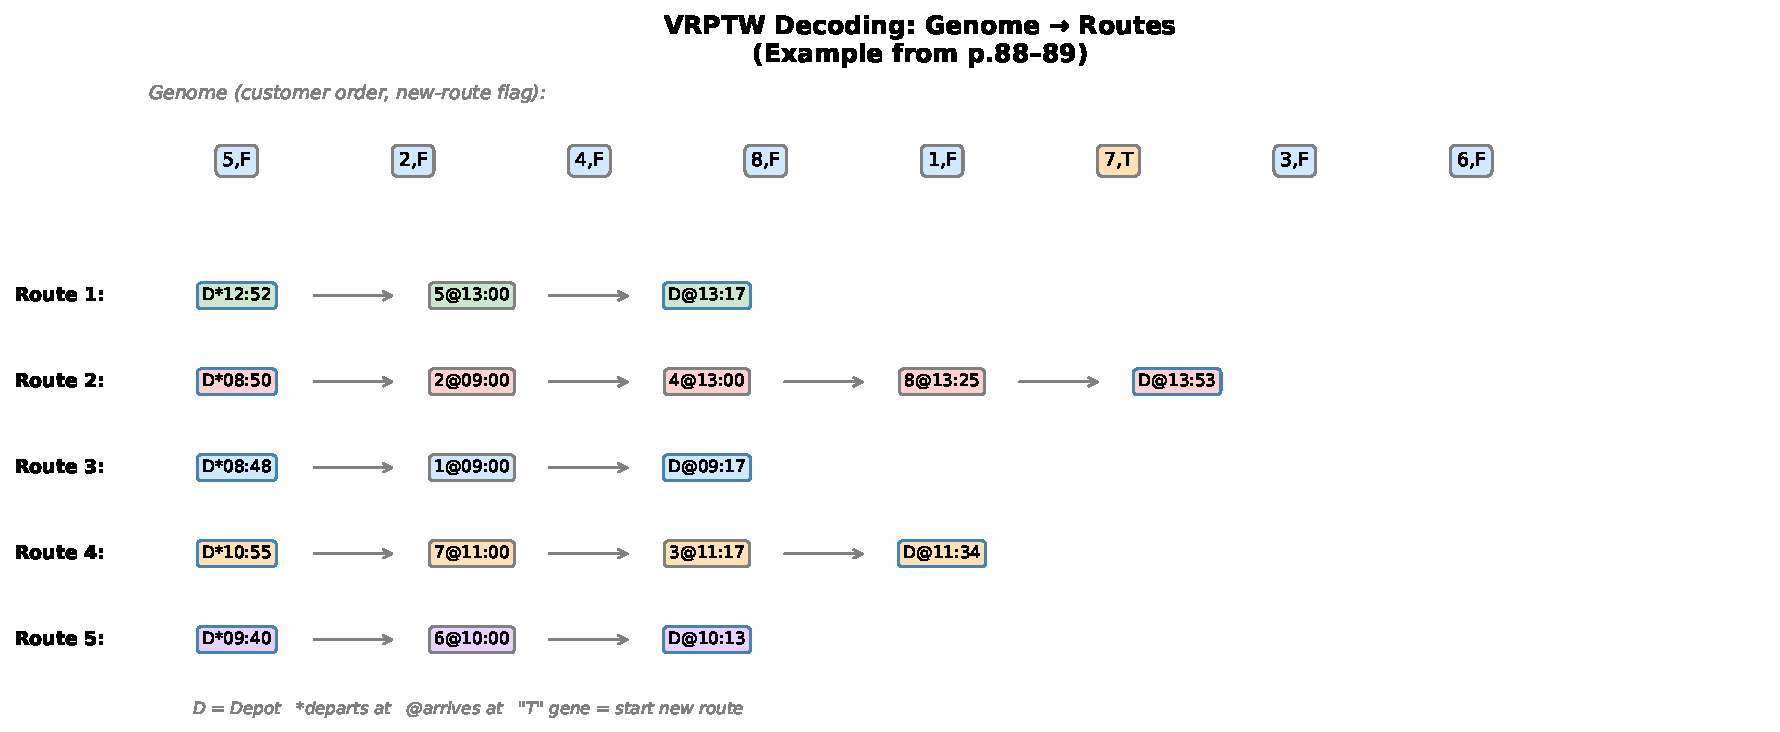
\includegraphics[width=0.92\textwidth]{fig_decoding_example.pdf}
    \caption{Visual summary of the genome-to-routes decoding process.
             The gene with flag T forces a new route regardless of
             feasibility.}
  \end{figure}

\end{frame}

% ────────────────────────────────────────────────────────────
\begin{frame}[fragile]{Python: VRPTW Decoder (Conceptual Implementation)}
% ────────────────────────────────────────────────────────────

  The core idea of the VRPTW decoder is straightforward to implement in Python.
  The following code demonstrates the logic used to translate a genome (ordered
  list of customers) into a set of routes while enforcing time windows and
  capacity constraints.

\begin{lstlisting}[caption={VRPTW Decoder in Python}]
SERVICE_TIME = 5   # minutes per customer visit
CAPACITY = 20      # maximum crates per vehicle
DEPOT_START = 8*60 + 30  # 08:30 in minutes since midnight

def decode_genome(genome, travel_times, windows, demands):
    """
    genome: list of (customer_id, new_route_flag) tuples
    travel_times: dict[(from, to)] -> minutes
    windows: dict[customer_id] -> (earliest, latest) in minutes
    demands: dict[customer_id] -> crates
    Returns: list of routes, each route = list of (customer, arrival_time)
    """
    routes = []
    current_route = []
    current_load = 0
    current_time = DEPOT_START
    current_pos = 'depot'

    for customer, new_route_flag in genome:
        travel = travel_times[(current_pos, customer)]
        arrival = current_time + travel

        # Check if we must start a new route
        must_split = (
            new_route_flag                        # gene flag forces new route
            or arrival > windows[customer][1]     # missed window (hard TW)
            or current_load + demands[customer] > CAPACITY  # capacity exceeded
        )

        if must_split and current_route:
            routes.append(current_route)
            current_route = []
            current_load = 0
            current_time = DEPOT_START  # new vehicle starts from depot
            current_pos = 'depot'
            travel = travel_times[('depot', customer)]
            arrival = current_time + travel

        # Wait if early
        service_start = max(arrival, windows[customer][0])
        depart_time = service_start + SERVICE_TIME

        current_route.append((customer, service_start))
        current_load += demands[customer]
        current_time = depart_time
        current_pos = customer

    if current_route:
        routes.append(current_route)

    return routes
\end{lstlisting}

\end{frame}

% ────────────────────────────────────────────────────────────
\begin{frame}[fragile]{Python: Single-Objective EA for VRPTW (from Book Listing 5.2)}
% ────────────────────────────────────────────────────────────

  The book implements the single-objective evolutionary algorithm for VRPTW in
  Java (Listing 5.2), but the logic translates directly to Python.  The algorithm
  maintains a population and uses tournament selection to pick parents and
  a ``worst'' individual to replace.

\begin{lstlisting}[caption={Single-Objective EA Main Loop (Java $\to$ Python translation)}]
import random

def solve_single_objective(problem, objective_fn, evals_budget=10000,
                           pop_size=50, tour_size=5, xo_rate=0.7):
    """
    Single-objective EA for VRPTW.
    objective_fn: callable(individual) -> float (minimise)
    Returns the best individual found.
    """
    population = [problem.random_individual() for _ in range(pop_size)]
    for ind in population:
        ind.evaluate(objective_fn)

    best_so_far = min(population, key=lambda x: x.fitness)
    budget = evals_budget

    while budget > 0:
        # Create child via crossover or mutation
        if random.random() < xo_rate:
            # Crossover: pick two parents by tournament
            p1 = tournament_select(population, tour_size)
            p2 = tournament_select(population, tour_size)
            child = p1.crossover(p2)
        else:
            # Mutation: copy one parent and mutate
            child = tournament_select(population, tour_size).copy()

        child.mutate()
        child.evaluate(objective_fn)
        budget -= 1

        # Replace worst individual if child is better
        worst = tournament_select_worst(population, tour_size)
        if worst.fitness > child.fitness:  # lower is better
            if child.fitness < best_so_far.fitness:
                best_so_far = child
            population.remove(worst)
            population.append(child)

    return best_so_far
\end{lstlisting}

\end{frame}

% ────────────────────────────────────────────────────────────
\begin{frame}[fragile]{Python: Home Delivery Solver (Algorithm 13)}
% ────────────────────────────────────────────────────────────

  Algorithm~13 (Home Delivery Solver) orchestrates the full solution
  process.  It runs the single-objective EA four times (once for each
  objective), runs the multi-objective EA ten times, pools all results,
  and extracts the grand Pareto front.

\begin{lstlisting}[caption={Home Delivery Solver — Python translation of Algorithm 13 / Listing 5.3}]
def home_delivery_solver(problem, n_tries=10):
    """
    Returns the grand non-dominated front (Pareto front) for the
    FabFoods VRPTW problem.
    """
    solution_pool = []

    # Phase 1: seed pool with single-objective optima (4 objectives)
    for _ in range(n_tries):
        for obj_fn in [cost_per_crate, total_distance,
                       total_time, num_routes]:
            best = solve_single_objective(problem, obj_fn)
            solution_pool.append(best)

    # Phase 2: run multi-objective EA many times
    for _ in range(n_tries):
        moea = NonDominatedEA(problem)
        moea.solve()
        solution_pool.extend(moea.get_non_dominated())

    # Phase 3: extract grand front from entire pool
    grand_front = extract_non_dominated(solution_pool)
    return grand_front


def extract_non_dominated(population):
    """Keep only solutions that are not dominated by any other."""
    front = []
    for candidate in population:
        dominated = any(
            dominates(other, candidate)
            for other in population
            if other is not candidate
        )
        if not dominated:
            front.append(candidate)
    return front


def dominates(a, b):
    """Solution a dominates b if a is at least as good on all objectives
    and strictly better on at least one."""
    objs_a = a.get_objectives()  # list of floats, all to minimise
    objs_b = b.get_objectives()
    at_least_as_good = all(oa <= ob for oa, ob in zip(objs_a, objs_b))
    strictly_better  = any(oa <  ob for oa, ob in zip(objs_a, objs_b))
    return at_least_as_good and strictly_better
\end{lstlisting}

\end{frame}

% ============================================================
\section{5.4 Finding Trade-Offs Using Pareto Dominance}
% ============================================================

\begin{frame}[allowframebreaks]{5.4 Finding Trade-Offs Using Pareto Dominance}

  To find the set of all \textbf{non-dominated trade-off solutions} we use the
  concept of \textbf{Pareto dominance}, introduced informally in Chapter 4 and
  formalised here for multiple objectives.

  \begin{block}{Definition: Pareto Dominance (Minimisation)}
    Let $\mathbf{f}(\mathbf{x}) = (f_1(\mathbf{x}), f_2(\mathbf{x}), \ldots,
    f_k(\mathbf{x}))$ denote the vector of $k$ (k) objective values of
    solution $\mathbf{x}$.  Solution $\mathbf{a}$ \textbf{dominates}
    solution $\mathbf{b}$ — written $\mathbf{a} \prec \mathbf{b}$ (prec,
    meaning ``is better than'') — if and only if:
    \begin{enumerate}
      \item $f_i(\mathbf{a}) \leq f_i(\mathbf{b})$ for \emph{all}
            $i = 1, \ldots, k$ (a is no worse on every objective), and
      \item $f_j(\mathbf{a}) < f_j(\mathbf{b})$ for \emph{at least one}
            $j$ (a is strictly better on at least one objective).
    \end{enumerate}
    A solution is \textbf{Pareto optimal} (non-dominated) if no other
    feasible solution dominates it.  The set of all Pareto-optimal
    solutions forms the \textbf{Pareto front}.
  \end{block}

  \begin{alertblock}{How to Read the Definition}
    Think of it this way: solution A dominates solution B if A is
    \emph{at least as good as B in every category} and
    \emph{strictly better in at least one category}.  If A delivers groceries
    for less cost, takes less time, needs fewer vehicles, and travels less
    distance than B, then A dominates B and B would never be chosen.
    The Pareto front consists of all solutions where any improvement in one
    dimension \emph{necessarily} comes at the cost of another.
  \end{alertblock}

\framebreak

  \begin{figure}
    \centering
    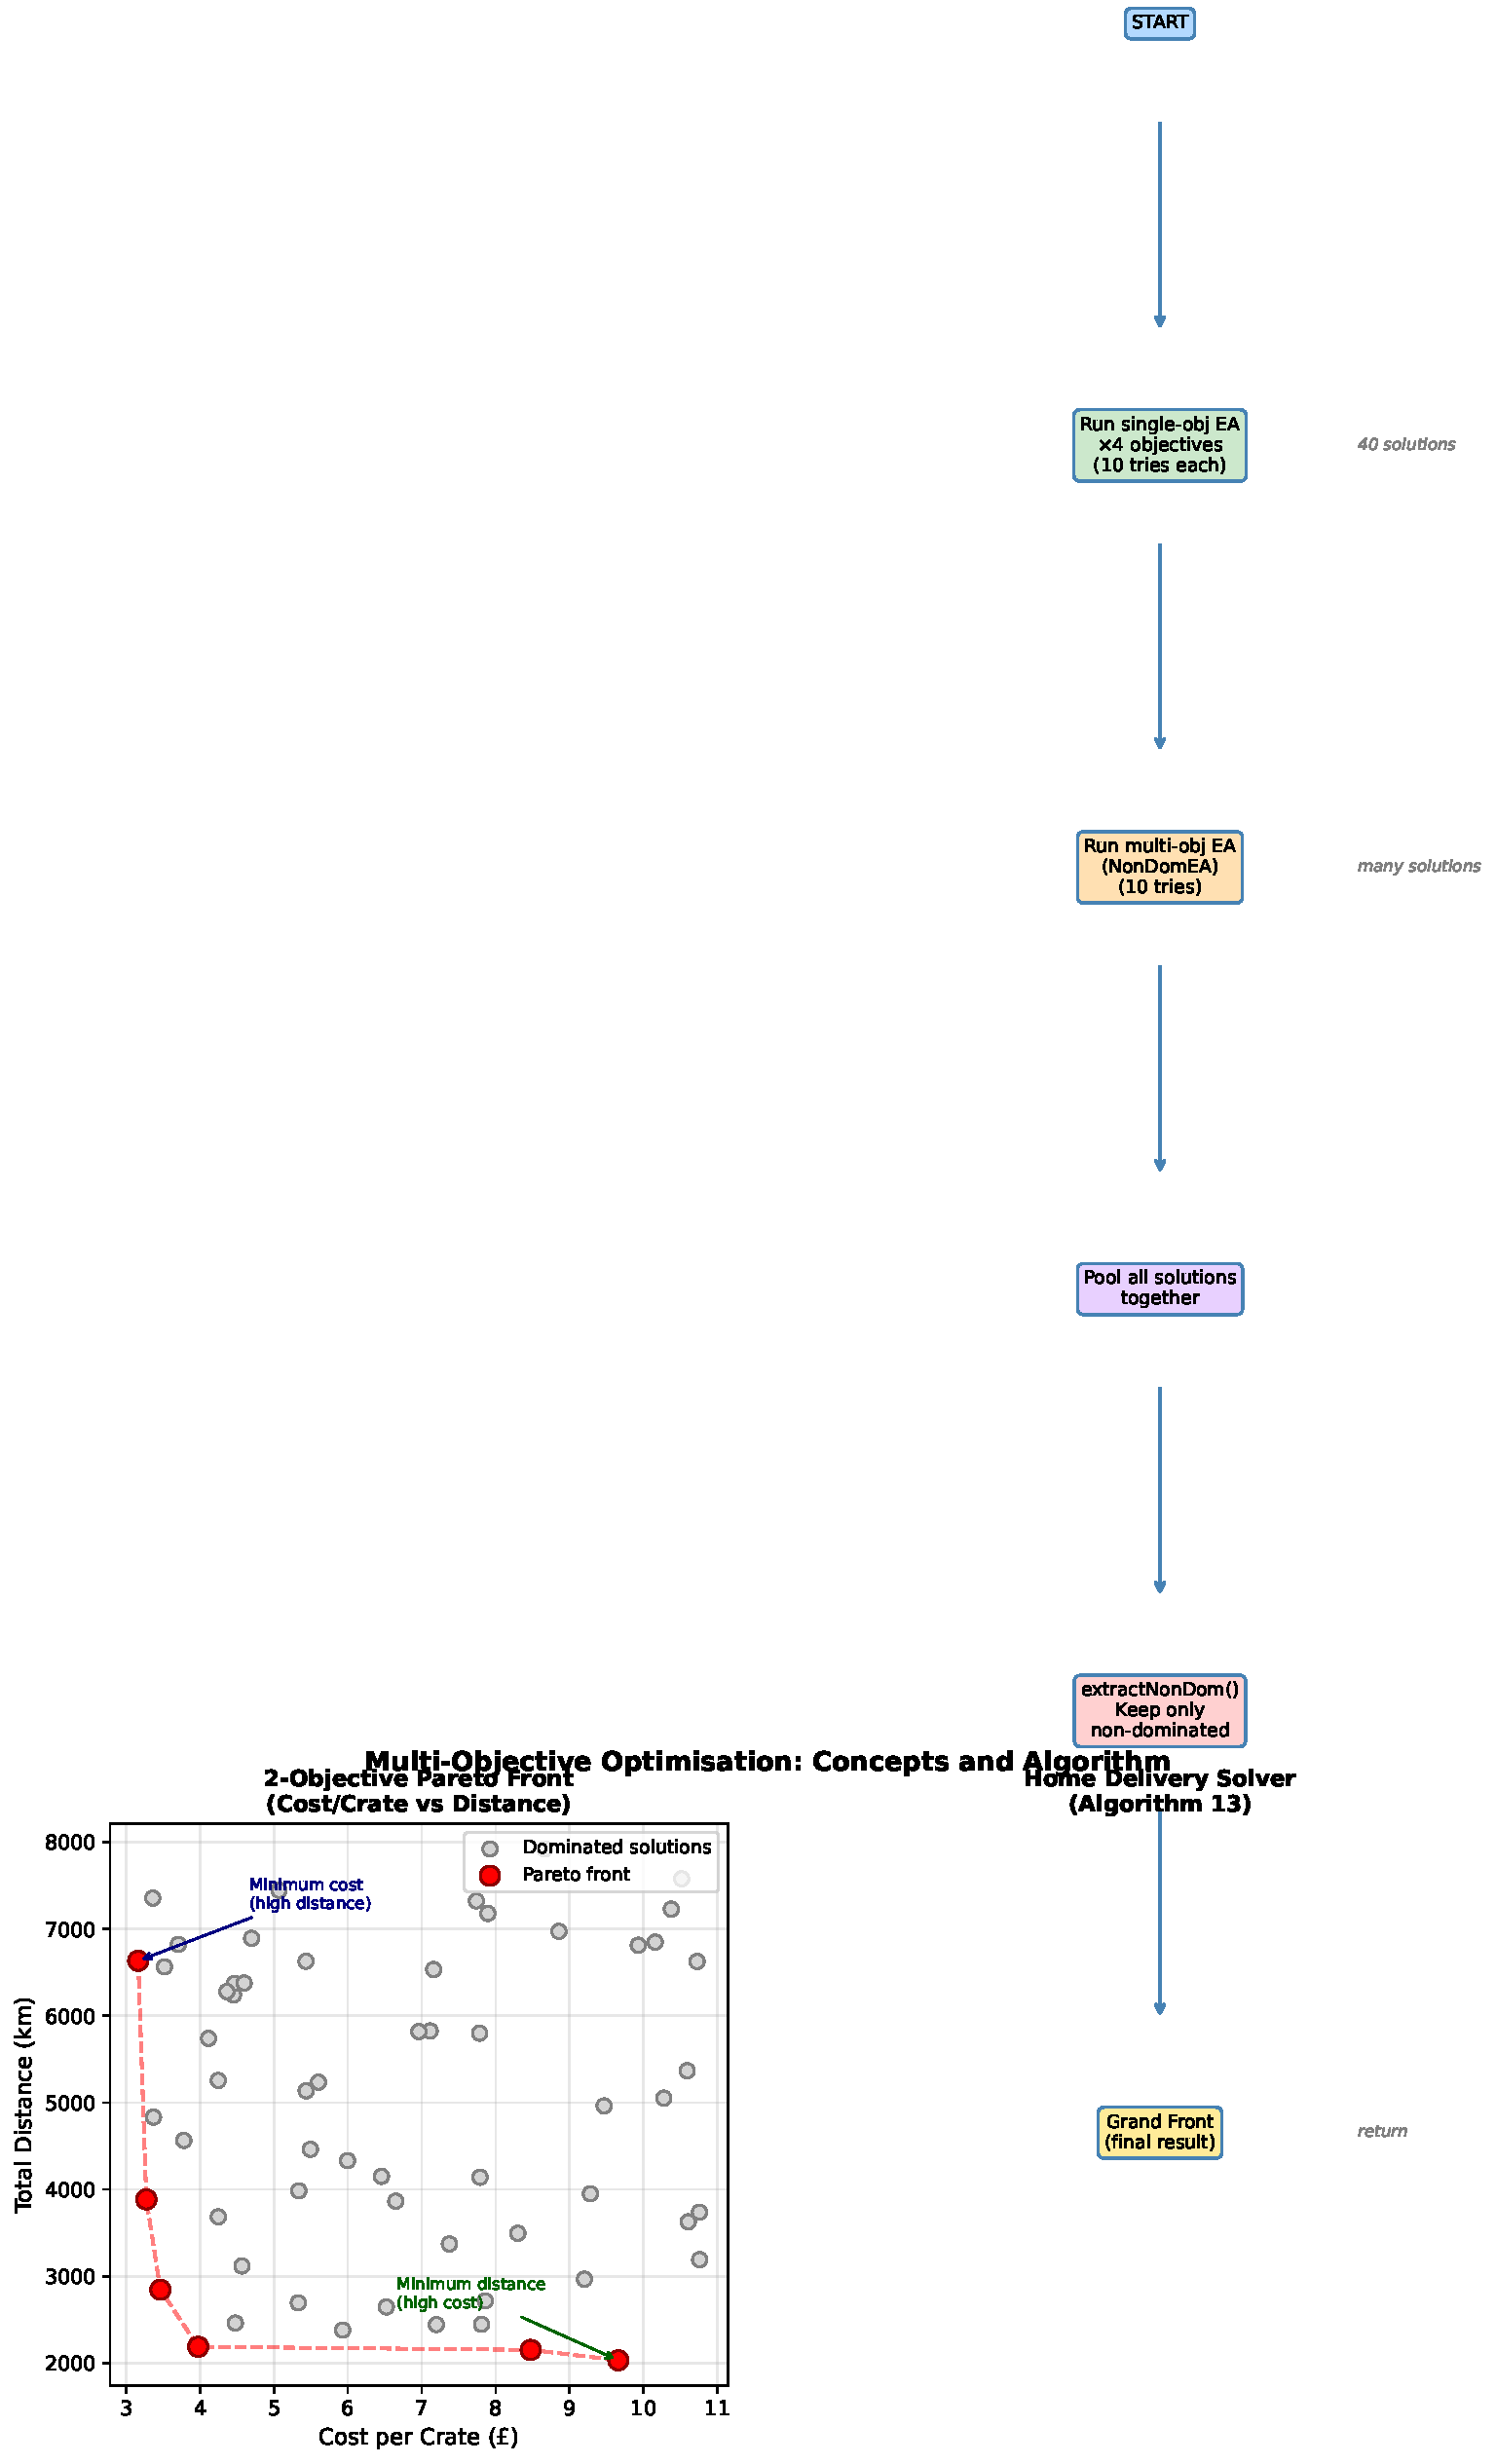
\includegraphics[width=0.90\textwidth]{fig_pareto_concept.pdf}
    \caption{Left: a 2-objective Pareto front for Cost/Crate vs Distance.
             Red dots are non-dominated solutions; grey dots are dominated.
             Right: the Home Delivery Solver (Algorithm~13) flow — first
             seeding the pool with single-objective optima, then running the
             multi-objective EA.}
  \end{figure}

\framebreak

  \begin{block}{The Hypervolume Indicator}
    The \textbf{hypervolume} (also called the $S$-metric) measures the
    quality of an entire Pareto front by computing the
    \textbf{volume of the objective space dominated by the front} relative
    to a fixed \emph{reference point} $\mathbf{r}$:
    \[
      HV(F, \mathbf{r}) = \lambda\!\left(\bigcup_{\mathbf{f} \in F}
        \{\mathbf{y} \mid \mathbf{f} \preceq \mathbf{y} \preceq \mathbf{r}\}
      \right)
    \]
    Here, $\lambda$ (lambda) denotes the Lebesgue measure (volume);
    $F$ is the Pareto front (set of objective vectors);
    $\mathbf{r}$ is a reference point that is worse than any solution
    on the front on all objectives; and $\preceq$ means
    ``component-wise less than or equal to.''

    A \textbf{larger hypervolume} is better: it means the front covers a
    wider and better region of objective space.
  \end{block}

  \begin{figure}
    \centering
    
\includegraphics[width=0.50\textwidth]{fig_hypervolume.pdf}
    \caption{The hypervolume is the shaded area dominated by the
             Pareto front (red dots) relative to the reference point
             (star).  A larger shaded area means a better front.}
  \end{figure}

\framebreak

  \begin{block}{Single-Objective Results (Seeding the Pool)}
    Before running the multi-objective EA, the book first solves each problem
    as four \emph{separate} single-objective problems.  This seeds the solution
    pool with ``extreme'' solutions that are guaranteed to be optimal (or
    near-optimal) for each individual objective.

    The results are reported in Tables 5.2, 5.3, and 5.4 across three
    benchmark sets (A, B, P) with time windows of 1 hour and 14 hours.
    Key findings:
    \begin{itemize}
      \item \textbf{A 1-hour time window roughly doubles the cost per crate}
            compared to a 14-hour window.  For example, on problem A-n32-k5,
            cost/crate rises from about \pounds 3.64 (14h) to \pounds 6.49 (1h).
      \item \textbf{Optimising on distance does not always give the lowest
            cost.}  The cost model includes a fixed per-vehicle charge, so
            saving distance can be offset by needing an extra vehicle.
      \item The optimal number of routes is \emph{known} for the Augerat
            benchmarks (it is part of the problem specification), allowing
            direct measurement of how many extra routes time windows impose.
    \end{itemize}
  \end{block}

  \begin{figure}
    \centering
    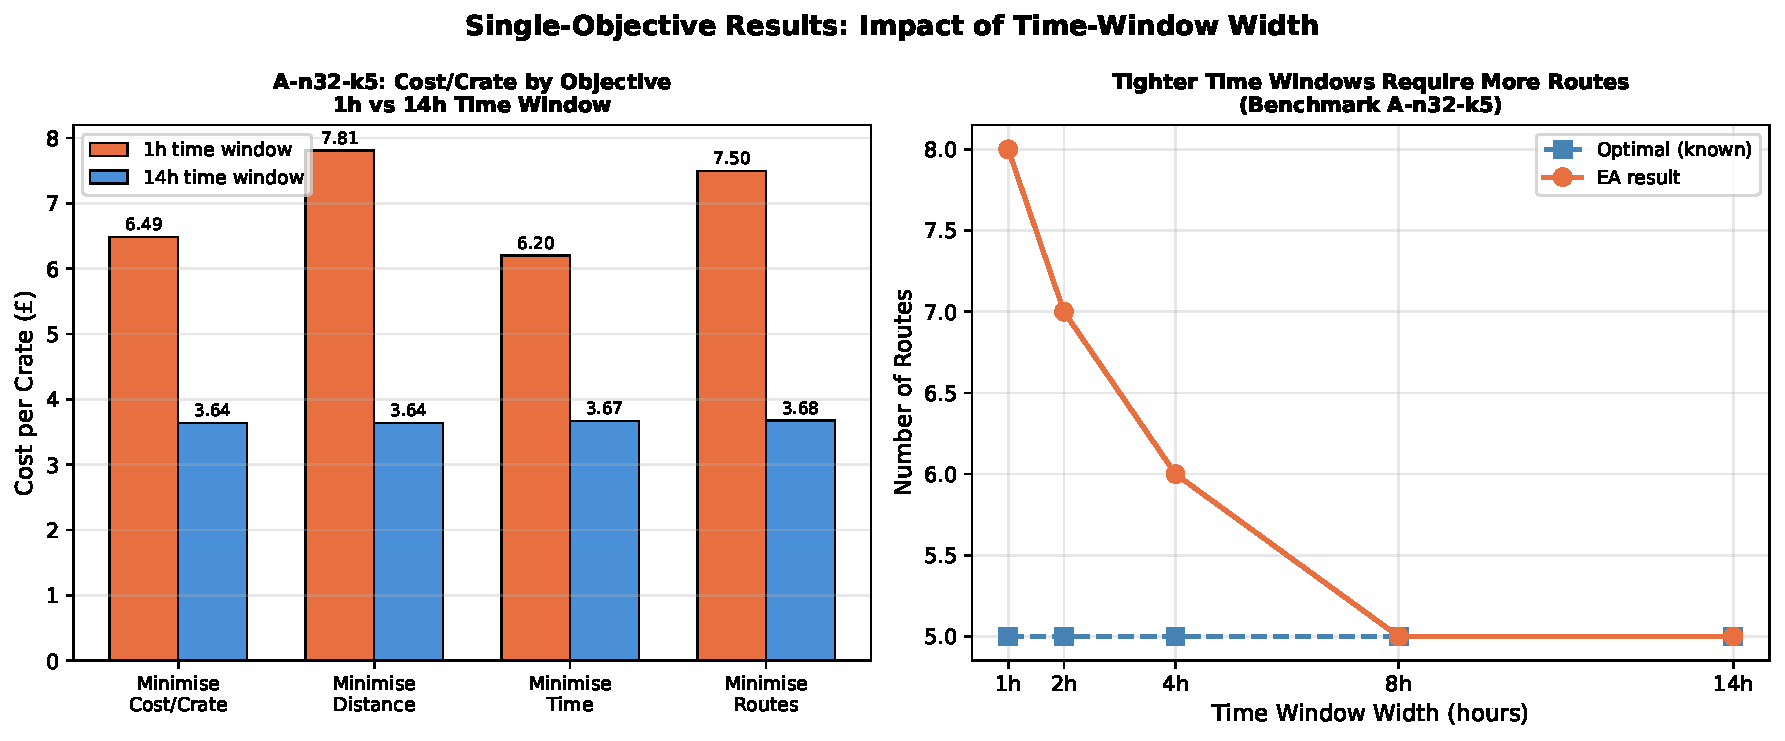
\includegraphics[width=0.82\textwidth]{fig_single_obj_results.pdf}
    \caption{Left: cost/crate when optimising each of the four objectives
             separately (A-n32-k5), comparing 1h and 14h time windows.
             Right: how the number of routes grows as the time window
             narrows.}
  \end{figure}

\framebreak

  \begin{block}{The Grand Pareto Front}
    After seeding the pool with single-objective optima, the multi-objective
    EA (NonDomEA) is run 10 times.  All solutions are pooled and the
    \texttt{extractNonDom()} procedure retains only the non-dominated ones.

    The size of this \textbf{grand front} (reported in Table 5.5) varies
    significantly with time-window width:
    \begin{itemize}
      \item With a \textbf{1-hour} time window, fronts typically contain
            \textbf{1--4 solutions} (very constrained, little room for
            trade-offs).
      \item With a \textbf{14-hour} time window, fronts are much larger
            (up to 85 solutions for some instances), reflecting genuine
            multi-dimensional trade-offs.
    \end{itemize}
  \end{block}

  \begin{exampleblock}{Worked Example: Grand Front for A-N32-K5 (14h TW)}
    The four initial single-objective solutions are:
    \begin{center}
    \small
    \begin{tabular}{lrrrr}
      \toprule
      Optimised for & Distance & Time & Cost/Crate & Routes \\
      \midrule
      Distance   & 2289.56 & 2014 & 3.64 & 5 \\
      Cost/Crate & 2557.11 & 2203 & 3.80 & 5 \\
      Routes     & 4112.92 & 3452 & 4.86 & 5 \\
      Time       & 2304.66 & 2099 & 3.68 & 5 \\
      \bottomrule
    \end{tabular}
    \end{center}
    After the MOEA runs and extracting the grand front, only \textbf{two}
    solutions remain:
    \begin{center}
    \small
    \begin{tabular}{rrrrll}
      \toprule
      Dist & Time & Cost/Crate & Routes & Notes \\
      \midrule
      2289.56 & 2014 & 3.64 & 5 & * single-obj distance solution \\
      2284.09 & 2079 & 3.67 & 5 & MOEA-found trade-off \\
      \bottomrule
    \end{tabular}
    \end{center}
    The MOEA found a solution (2284.09 km) that \textbf{dominates the original
    distance optimum} (2289.56 km) on distance while having slightly higher
    time (2079 vs 2014) and slightly higher cost/crate (3.67 vs 3.64).
    Actually the MOEA solution has \emph{lower} distance, meaning it dominates
    the single-objective distance solution on distance.
  \end{exampleblock}

\framebreak

  \begin{block}{Hypervolume Comparison: 14h vs 1h Time Windows (Table 5.6)}
    Table 5.6 reports the hypervolume values for each problem instance under
    both time-window settings.  The key finding is dramatic:

    \begin{center}
    \small
    \begin{tabular}{lrr}
      \toprule
      Problem & HV (1h window) & HV (14h window) \\
      \midrule
      A-n32-k5 & 6,914,025 & 90,211,910 \\
      A-n33-k5 & 21,411,225 & 165,201,964 \\
      A-n34-k5 & 1,650,146 & 341,571,126 \\
      A-n36-k5 & 7,086,072 & 188,364,509 \\
      \bottomrule
    \end{tabular}
    \end{center}

    The 14-hour window consistently produces hypervolumes that are
    \textbf{10$\times$ to 100$\times$ larger} than the 1-hour window.
    This confirms that tight time windows severely restrict the diversity
    of solutions available to the decision-maker: there are simply fewer
    feasible solutions when constraints are tight, leaving little room for
    Pareto-optimal trade-offs.
  \end{block}

\end{frame}

% ============================================================
\section{5.5 Exploring Many-Dimensional Fronts}
% ============================================================

\begin{frame}[allowframebreaks]{5.5 Exploring Many-Dimensional Fronts}

  When the Pareto front contains many solutions across four dimensions, it
  is impossible to display it as a simple 2D scatter plot.  We need a
  richer visualisation.  The technique introduced in this section is the
  \textbf{Parallel Coordinates plot} (Inselberg 2009).

  \begin{block}{What Is a Parallel Coordinates Plot?}
    A parallel coordinates (PC) plot represents multi-dimensional data as
    follows:
    \begin{itemize}
      \item Draw one \textbf{vertical axis} for each dimension (objective).
            For our four-objective problem there are four axes: Distance,
            Time, Cost/Crate, and Routes.
      \item Each \textbf{axis is scaled} from its minimum to its maximum value
            across all solutions.
      \item Represent each \textbf{solution as a poly-line} — a broken line
            that crosses each axis at the value of that solution on that
            objective.
      \item A solution that is good on all objectives will be low on all axes
            (since we are minimising); a solution that is good on cost but
            poor on distance will be low on the cost axis and high on the
            distance axis.
    \end{itemize}
  \end{block}

\framebreak

  \begin{figure}
    \centering
    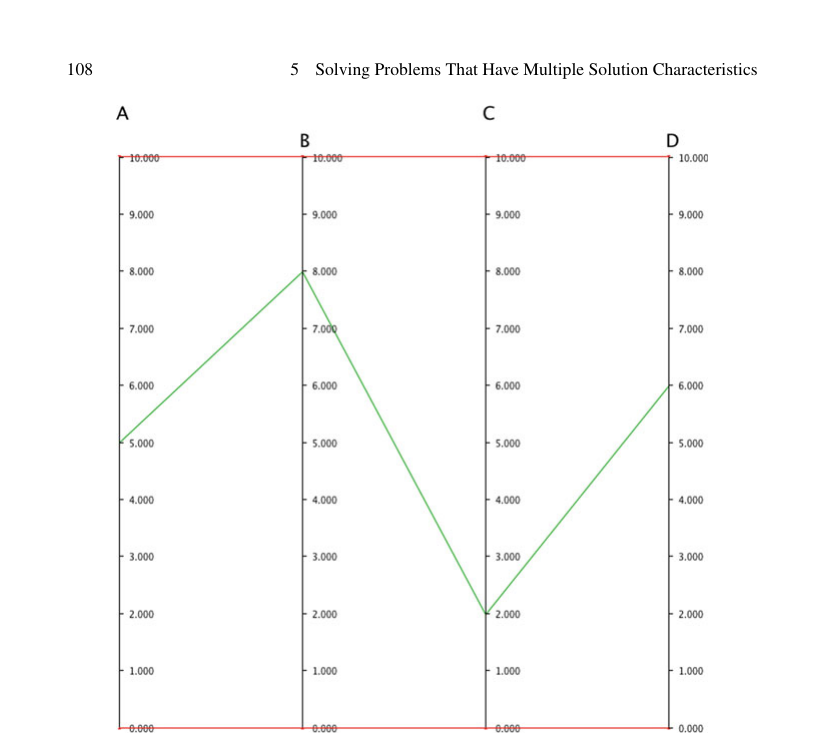
\includegraphics[width=0.60\textwidth]{fig_crop_pc_single_point.png}
    \caption{Fig.~5.1 from the book: a single 4-dimensional point $(5, 8, 2, 6)$
             plotted on a parallel coordinates plot with axes $A$, $B$, $C$, $D$.
             The point is shown as a single poly-line intersecting each axis
             at the appropriate value.}
  \end{figure}

  The key observation is that a point in 4D space becomes a \textbf{path}
  through four vertical lines.  When many solutions are plotted together, the
  resulting ``tangle'' of lines reveals patterns: clusters of similar solutions,
  trade-off relationships (a line going up on one axis typically goes down on
  another), and outliers.

\framebreak

  \begin{block}{The Grand Front for B-n78-k10 (1h Time Windows)}
    Table 5.7 lists all 17 non-dominated solutions for problem B-n78-k10
    with a 1-hour time window.  All four objectives are listed:
  \end{block}

  \begin{center}
  \small
  \begin{tabular}{rrrrrr}
    \toprule
    Sol.\ \# & Distance & Time & Cost/Crate & Routes & Notes \\
    \midrule
    1  & 7134.90 & 8294 & 10.01 & 42 & High cost \\
    3  & 6506.86 & 8539 &  7.71 & 29 & \\
    9  & 6257.10 & 8573 &  7.16 & 26 & \\
    12 & 6188.65 & 8804 &  6.50 & 22 & \\
    14 & 6029.59 & 9126 &  6.73 & 23 & \\
    15 & 6196.21 & 9045 &  6.38 & 21 & \textbf{Lowest cost/crate} \\
    17 & 6057.71 & 9118 &  6.55 & 22 & \\
    \bottomrule
    \multicolumn{6}{l}{\footnotesize (Abbreviated; full table has 17 rows)}
  \end{tabular}
  \end{center}

  Notice the clear trade-off: solutions with lower cost/crate (e.g.,
  solution 15 at \pounds 6.38/crate) tend to have \textbf{higher time} values
  (9045 minutes).  This is because reducing the number of routes (21 vs 42)
  saves vehicle costs but forces drivers to take longer routes.

\framebreak

  \begin{figure}
    \centering
    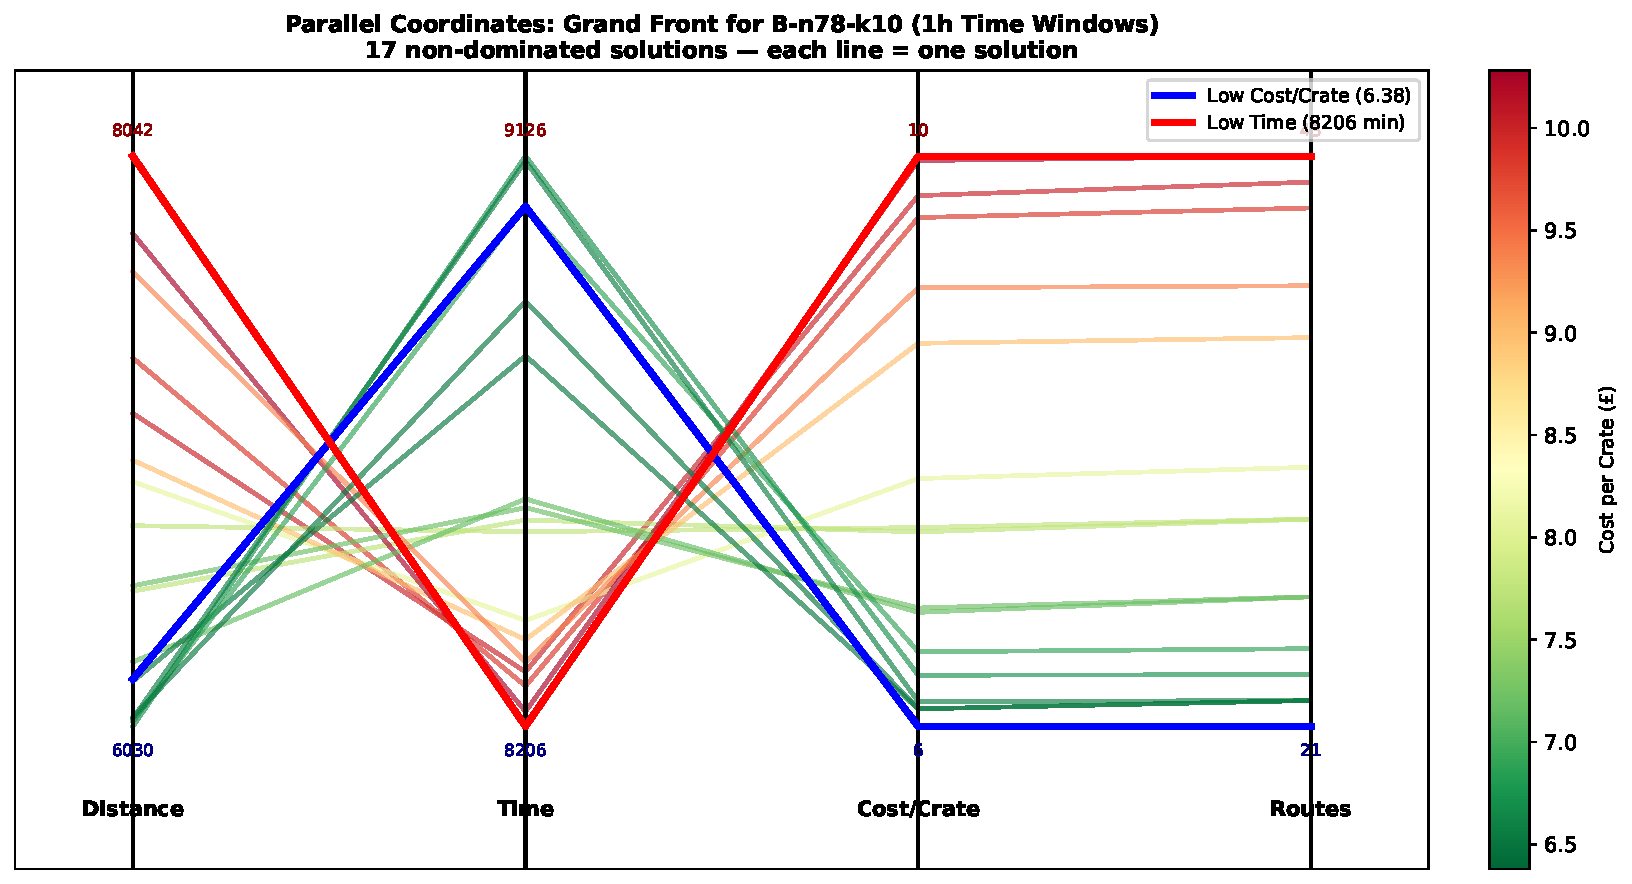
\includegraphics[width=0.88\textwidth]{fig_parallel_coords.pdf}
    \caption{Parallel coordinates plot of all 17 non-dominated solutions
             for B-n78-k10 (1h TW).  Each line is one solution.
             Colour indicates cost per crate (green = low, red = high).
             The blue line highlights the lowest-cost solution;
             the red line highlights the fastest solution.}
  \end{figure}

\framebreak

  \begin{block}{Using Filters to Find a Trade-Off Solution}
    The real power of parallel coordinates is \textbf{interactive filtering}.
    A filter restricts which solutions are highlighted by specifying an
    acceptable range on one or more axes.  Only solutions whose poly-lines
    pass through all active filter ranges are highlighted.

    \textbf{Scenario:} A manager at FabFoods has been told to reduce
    cost/crate, but has also received complaints about long delivery times.
    The manager applies two filters:
    \begin{enumerate}
      \item \textbf{Filter 1 — Cost/Crate $\leq$ 7.0}: highlights solutions
            with low delivery cost.
      \item \textbf{Filter 2 — Time $\leq$ 9000 minutes}: further restricts
            to solutions that also have lower total route time.
    \end{enumerate}
    The intersection of both filters reveals the trade-off solutions that
    satisfy both constraints simultaneously.
  \end{block}

  \begin{figure}
    \centering
    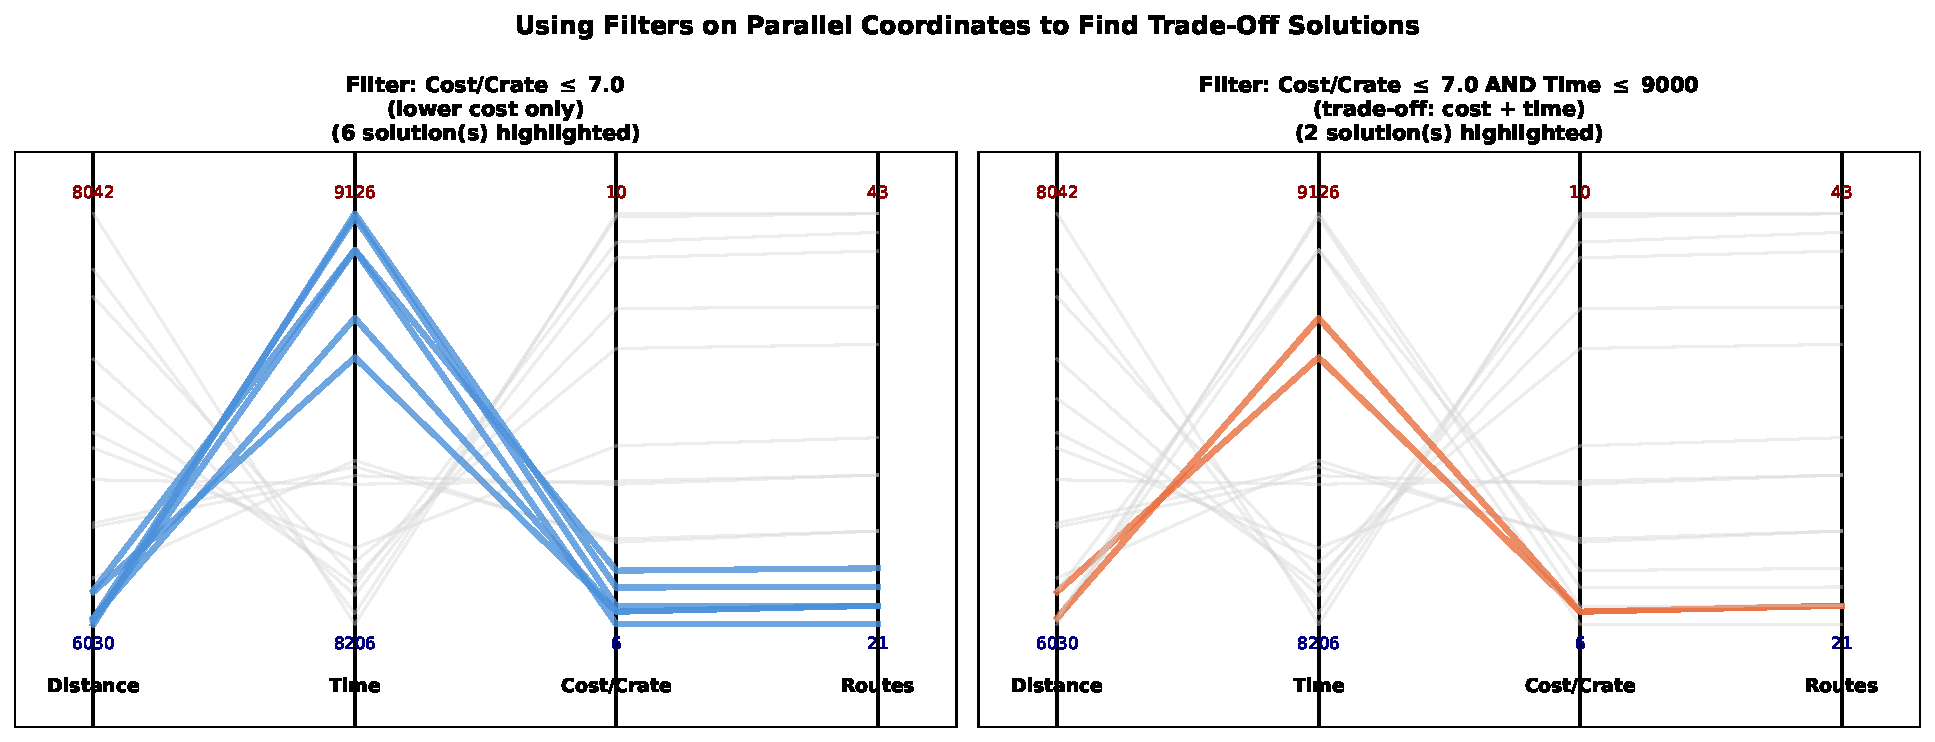
\includegraphics[width=0.90\textwidth]{fig_parallel_coords_filter.pdf}
    \caption{Left: applying Filter 1 (low cost/crate $\leq 7.0$) highlights
             several solutions.  Right: adding Filter 2 (time $\leq 9000$
             min) narrows the choice to a single solution that balances both
             concerns.  Unselected lines are grey.}
  \end{figure}

\framebreak

  \begin{figure}
    \centering
    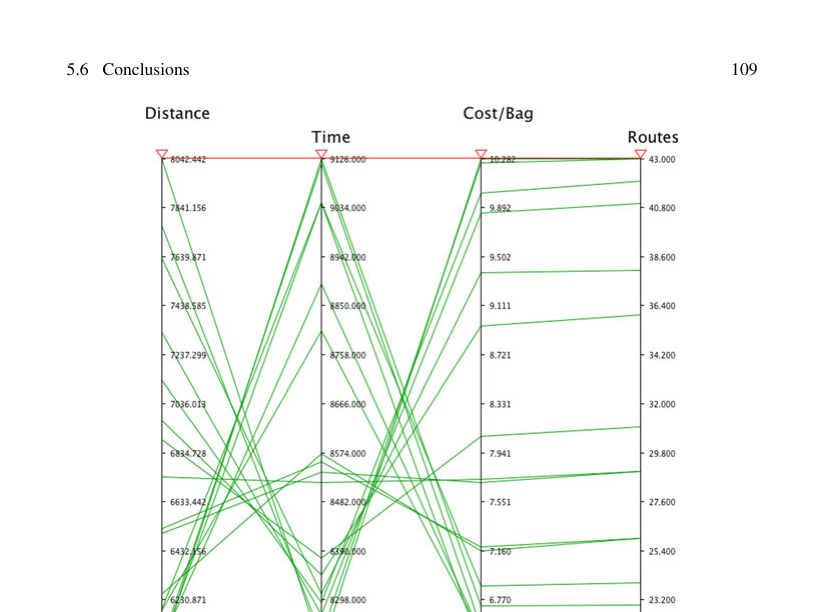
\includegraphics[width=0.75\textwidth]{fig_crop_pc_all_solutions.png}
    \caption{Fig.~5.2 from the book: all 17 non-dominated solutions from
             Table 5.7 plotted together using the XDat application.
             The axes are Distance, Time, Cost/Bag, and Routes (left to right).}
  \end{figure}

  \begin{figure}
    \centering
    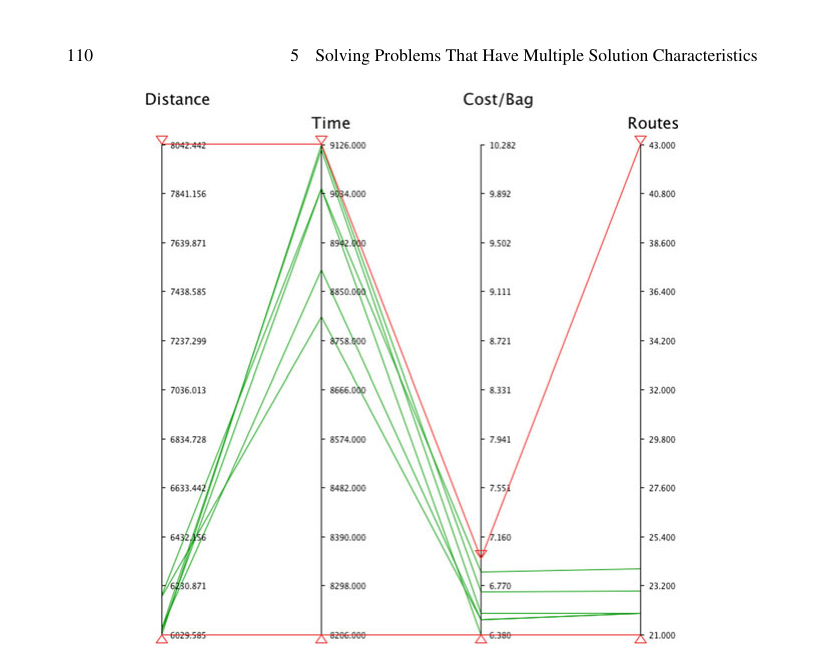
\includegraphics[width=0.75\textwidth]{fig_crop_pc_filter_cost.png}
    \caption{Fig.~5.3 from the book: applying a filter on the low end of
             Cost/Crate axis.  The highlighted green lines show solutions
             with lower cost — notice they tend to have higher Time values,
             confirming the cost-vs-time trade-off.}
  \end{figure}

\framebreak

  \begin{figure}
    \centering
    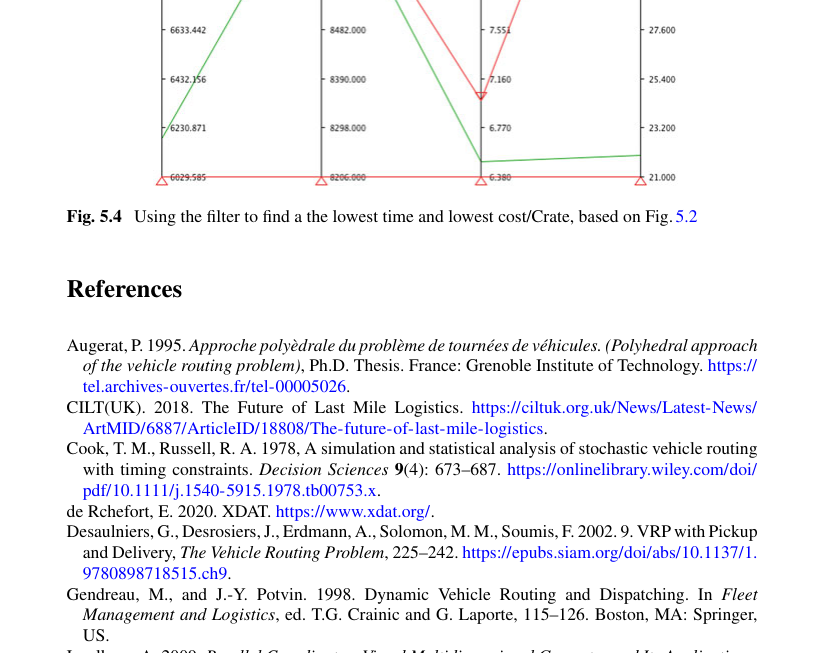
\includegraphics[width=0.75\textwidth]{fig_crop_pc_filter_both.png}
    \caption{Fig.~5.4 from the book: a further filter is applied to the Time
             axis to highlight solutions with both lower cost/crate and
             lower time.  Only the solutions passing through both filter
             regions remain highlighted, giving the manager a small
             shortlist of trade-off solutions.}
  \end{figure}

\framebreak

  \begin{alertblock}{Key Insight: Parallel Coordinates for Decision Support}
    The parallel coordinates plot does not make the decision for the manager
    — that remains a human judgment.  Instead, it \textbf{informs} the
    decision by making trade-offs visible and filterable.  The approach was
    motivated by a real conversation: when the author first presented a
    non-dominated set of 500 solutions to a transportation planner, the
    planner pointed out that choosing from 500 options was itself a hard
    problem.  The interactive visualisation resolves this by letting the
    planner \textbf{express constraints interactively} and see immediately
    which solutions satisfy them.
  \end{alertblock}

  \begin{block}{Practical Notes on Parallel Coordinates}
    \begin{itemize}
      \item The \textbf{order of axes} matters: trade-offs between
            adjacent axes are easiest to see (crossing lines between two
            axes indicate a conflict).
      \item Axes can be \textbf{normalised} to $[0,1]$ or kept in their
            natural units; normalisation allows visual comparison across
            objectives of different magnitudes.
      \item The book uses the \textbf{XDat} application for interactive
            filtering; Python implementations include the
            \texttt{pandas} \texttt{parallel\_coordinates} function and
            the \texttt{plotly} library.
    \end{itemize}
  \end{block}

\end{frame}

% ────────────────────────────────────────────────────────────
\begin{frame}[fragile]{Python: Parallel Coordinates Plot with Filtering}
% ────────────────────────────────────────────────────────────

  The following Python code reproduces the parallel coordinates plot from
  Figure 5.2 of the book and demonstrates how to apply filters programmatically.

\begin{lstlisting}[caption={Parallel Coordinates with Filters (Python/matplotlib)}]
import numpy as np
import matplotlib.pyplot as plt

def parallel_coords_with_filter(solutions, axis_names,
                                filters=None, highlight_color='blue'):
    """
    solutions: numpy array of shape (n_solutions, n_objectives)
    axis_names: list of objective names
    filters: list of (axis_index, min_val, max_val) tuples
    """
    n_sol, n_dim = solutions.shape
    mins = solutions.min(axis=0)
    maxs = solutions.max(axis=0)
    norm = (solutions - mins) / (maxs - mins + 1e-9)  # normalise to [0,1]

    fig, ax = plt.subplots(figsize=(10, 5))
    x = np.arange(n_dim)

    # Determine which solutions pass all filters
    if filters:
        passes = np.ones(n_sol, dtype=bool)
        for (axis_idx, fmin, fmax) in filters:
            passes &= ((solutions[:, axis_idx] >= fmin) &
                       (solutions[:, axis_idx] <= fmax))
    else:
        passes = np.ones(n_sol, dtype=bool)

    for i, row in enumerate(norm):
        color = highlight_color if passes[i] else 'lightgray'
        alpha = 0.8 if passes[i] else 0.3
        lw = 2.5 if passes[i] else 1.0
        ax.plot(x, row, color=color, alpha=alpha, linewidth=lw)

    for j, name in enumerate(axis_names):
        ax.axvline(j, color='black', linewidth=1.5)
        ax.text(j, 1.05, f'{maxs[j]:.0f}', ha='center', fontsize=8)
        ax.text(j, -0.05, f'{mins[j]:.0f}', ha='center', fontsize=8)
        ax.text(j, -0.15, name, ha='center', fontsize=10, fontweight='bold')

    ax.set_xlim(-0.2, n_dim - 0.8)
    ax.set_ylim(-0.2, 1.1)
    ax.set_xticks([]); ax.set_yticks([])
    n_shown = passes.sum()
    ax.set_title(f'Parallel Coordinates: {n_shown}/{n_sol} solutions shown')
    plt.tight_layout()
    plt.savefig('pareto_front_parallel.pdf', bbox_inches='tight')
    return fig

# Example: filter to low cost/crate (column 2) and low time (column 1)
solutions = np.array([  # Table 5.7 data (Distance, Time, Cost/Crate, Routes)
    [7134.9, 8294, 10.01, 42],
    [6506.86, 8539, 7.71, 29],
    [6257.1, 8573, 7.16, 26],
    [6188.65, 8804, 6.5, 22],
    [6196.21, 9045, 6.38, 21],
    # ... (all 17 solutions)
])
filters = [(2, 0, 7.0), (1, 0, 9000)]  # Cost/Crate <= 7.0, Time <= 9000
parallel_coords_with_filter(solutions, ['Distance','Time','Cost/Crate','Routes'],
                            filters=filters, highlight_color='orange')
\end{lstlisting}

\end{frame}

% ============================================================
\section{5.6 Conclusions}
% ============================================================

\begin{frame}[allowframebreaks]{5.6 Conclusions}

  This chapter has demonstrated that real-world delivery problems are
  inherently multi-objective.  The key contributions and takeaways are
  summarised below.

  \begin{block}{What Was Introduced}
    \begin{enumerate}
      \item \textbf{The VRPTW formulation.}  By adding time-window
            constraints to the VRP, the problem becomes significantly harder:
            tight windows can double the required number of routes and the
            associated cost.  The decoder must handle waiting time, service
            time, and the possibility of route splitting when windows are
            missed.
      \item \textbf{The FabFoods cost model.}  A realistic four-component
            cost model (fixed vehicle cost, per-km running cost, staff time
            cost, and cost-per-crate) grounds the optimisation in real
            financial terms.
      \item \textbf{The Home Delivery Solver (Algorithm 13).}  A two-phase
            approach: seed a solution pool with single-objective optima
            (one for each of the four objectives), then run the
            multi-objective EA repeatedly and extract the non-dominated
            grand front.
    \end{enumerate}
  \end{block}

\framebreak

  \begin{block}{What Was Demonstrated}
    \begin{itemize}
      \item \textbf{Why evolutionary algorithms suit multi-objective
            problems.}  Because EAs maintain a \emph{population}, they
            naturally produce many trade-off solutions in a single run —
            something impossible with single-solution methods like hill
            climbing.
      \item \textbf{The effect of time-window width.}  The hypervolume
            results (Table 5.6) show that 14-hour windows produce fronts
            with 10$\times$--100$\times$ larger hypervolume than 1-hour
            windows, meaning a far richer set of trade-offs is available.
      \item \textbf{Parallel coordinates for decision support.}  When a
            Pareto front has many solutions and many objectives, interactive
            filtering on a parallel coordinates plot allows a decision-maker
            to express preferences one constraint at a time and quickly
            narrow the choice to a practical shortlist.
    \end{itemize}
  \end{block}

  \begin{alertblock}{The Big Picture}
    Multi-objective optimisation does not replace human judgment — it
    enhances it.  The algorithm's job is to find the \emph{frontier of
    possibilities}; the decision-maker's job is to \emph{choose a point on
    that frontier} based on priorities that may be difficult to quantify
    in advance.  Parallel coordinates and similar visualisation tools are
    the bridge between algorithmic output and human decision-making.
  \end{alertblock}

\framebreak

  \begin{block}{Connections to the Rest of the Book}
    \begin{itemize}
      \item \textbf{Chapter 2} introduced the VRP representation and the
            permutation-with-breaks encoding used here.
      \item \textbf{Chapter 4} introduced Pareto dominance for two
            objectives; this chapter generalises it to four.
      \item Future chapters build on the multi-objective framework to
            handle even more complex real-world scenarios.
    \end{itemize}
  \end{block}

  \begin{block}{Further Reading}
    \begin{itemize}
      \item Solomon, M.M.\ (1987). Algorithms for the vehicle routing and
            scheduling problems with time window constraints.
            \textit{Operations Research} 35(2): 254--265.
      \item Inselberg, A.\ (2009). \textit{Parallel Coordinates: Visual
            Multidimensional Geometry and Its Applications}.
            Springer.
      \item Augerat, P.\ (1995). \textit{Approche polyèdrale du problème
            de tournées de véhicules}.  Ph.D.\ Thesis, Grenoble INP.
      \item de Rchefort, G.\ (2020). XDat application for parallel
            coordinates visualisation. \url{https://www.xdat.org/}
    \end{itemize}
  \end{block}

\end{frame}

% ────────────────────────────────────────────────────────────
\begin{frame}{Summary: Chapter 5 at a Glance}
% ────────────────────────────────────────────────────────────

  \begin{columns}[t]
    \column{0.48\textwidth}
    \begin{block}{Key Concepts}
      \begin{itemize}
        \item \textbf{Last mile}: final delivery to consumer home;
              multi-objective by nature.
        \item \textbf{VRPTW}: VRP + time windows; hard window
              $\Rightarrow$ infeasible if late; soft window
              $\Rightarrow$ penalty.
        \item \textbf{Pareto dominance}: A dominates B if A is
              no worse on all objectives and strictly better on at
              least one.
        \item \textbf{Grand Pareto front}: union of all non-dominated
              solutions from both single- and multi-objective runs.
        \item \textbf{Hypervolume}: area/volume of objective space
              dominated by the front; larger = better front.
        \item \textbf{Parallel coordinates}: visualise $n$-D fronts
              as poly-lines; filter axes to find trade-offs.
      \end{itemize}
    \end{block}

    \column{0.48\textwidth}
    \begin{block}{Key Formulas}
      \small
      \textbf{Vehicle cost:}
      $\text{noRoutes} \times 164 + \text{dist} \times 0.117$

      \medskip
      \textbf{Staff cost:}
      $\text{totalTime(hrs)} \times 12$

      \medskip
      \textbf{Cost per crate:}
      $\dfrac{\text{vehicleCost} + \text{staffCost}}{\text{totalDemand}}$

      \medskip
      \textbf{Pareto dominance} ($\mathbf{a} \prec \mathbf{b}$):
      $f_i(a) \leq f_i(b)\ \forall i$ and $\exists j: f_j(a) < f_j(b)$

      \medskip
      \textbf{Algorithm 13 flow:}\\
      Single-obj $\times 4$ (10 tries each)
      $\to$ MOEA (10 tries)
      $\to$ \texttt{extractNonDom}
      $\to$ Grand Front
    \end{block}
  \end{columns}

  \vspace{0.3em}
  \begin{alertblock}{Final Takeaway}
    Evolutionary algorithms are \textbf{population-based} and therefore
    naturally explore the Pareto front in a single run.  Combined with
    \textbf{visualisation tools} like parallel coordinates, they transform
    a massive optimisation problem into an actionable set of options
    for a human decision-maker.
  \end{alertblock}

\end{frame}

\end{document}
